\documentclass[journal,12pt,twocolumn]{IEEEtran}

\usepackage{setspace}
\usepackage{gensymb}

\singlespacing


\usepackage[cmex10]{amsmath}

\usepackage{amsthm}

\usepackage{mathrsfs}
\usepackage{txfonts}
\usepackage{stfloats}
\usepackage{bm}
\usepackage{cite}
\usepackage{cases}
\usepackage{subfig}

\usepackage{longtable}
\usepackage{multirow}

\usepackage{enumitem}
\usepackage{mathtools}
\usepackage{steinmetz}
\usepackage{tikz}
\usepackage{circuitikz}
\usepackage{verbatim}
\usepackage{tfrupee}
\usepackage[breaklinks=true]{hyperref}
\usepackage{graphicx}
\usepackage{tkz-euclide}
\usepackage{float}

\usetikzlibrary{calc,math}
\usepackage{listings}
    \usepackage{color}                                            %%
    \usepackage{array}                                            %%
    \usepackage{longtable}                                        %%
    \usepackage{calc}                                             %%
    \usepackage{multirow}                                         %%
    \usepackage{hhline}                                           %%
    \usepackage{ifthen}                                           %%
    \usepackage{lscape}     
\usepackage{multicol}
\usepackage{chngcntr}

\DeclareMathOperator*{\Res}{Res}

\renewcommand\thesection{\arabic{section}}
\renewcommand\thesubsection{\thesection.\arabic{subsection}}
\renewcommand\thesubsubsection{\thesubsection.\arabic{subsubsection}}

\renewcommand\thesectiondis{\arabic{section}}
\renewcommand\thesubsectiondis{\thesectiondis.\arabic{subsection}}
\renewcommand\thesubsubsectiondis{\thesubsectiondis.\arabic{subsubsection}}


\hyphenation{op-tical net-works semi-conduc-tor}
\def\inputGnumericTable{}                                 %%

\lstset{
%language=C,
frame=single, 
breaklines=true,
columns=fullflexible
}
\begin{document}


\newtheorem{theorem}{Theorem}[section]
\newtheorem{problem}{Problem}
\newtheorem{proposition}{Proposition}[section]
\newtheorem{lemma}{Lemma}[section]
\newtheorem{corollary}[theorem]{Corollary}
\newtheorem{example}{Example}[section]
\newtheorem{definition}[problem]{Definition}

\newcommand{\BEQA}{\begin{eqnarray}}
\newcommand{\EEQA}{\end{eqnarray}}
\newcommand{\define}{\stackrel{\triangle}{=}}
\bibliographystyle{IEEEtran}
\providecommand{\mbf}{\mathbf}
\providecommand{\pr}[1]{\ensuremath{\Pr\left(#1\right)}}
\providecommand{\qfunc}[1]{\ensuremath{Q\left(#1\right)}}
\providecommand{\sbrak}[1]{\ensuremath{{}\left[#1\right]}}
\providecommand{\lsbrak}[1]{\ensuremath{{}\left[#1\right.}}
\providecommand{\rsbrak}[1]{\ensuremath{{}\left.#1\right]}}
\providecommand{\brak}[1]{\ensuremath{\left(#1\right)}}
\providecommand{\lbrak}[1]{\ensuremath{\left(#1\right.}}
\providecommand{\rbrak}[1]{\ensuremath{\left.#1\right)}}
\providecommand{\cbrak}[1]{\ensuremath{\left\{#1\right\}}}
\providecommand{\lcbrak}[1]{\ensuremath{\left\{#1\right.}}
\providecommand{\rcbrak}[1]{\ensuremath{\left.#1\right\}}}
\theoremstyle{remark}
\newtheorem{rem}{Remark}
\newcommand{\sgn}{\mathop{\mathrm{sgn}}}
\providecommand{\abs}[1]{\lvert#1\vert}
\providecommand{\res}[1]{\Res\displaylimits_{#1}} 
\providecommand{\norm}[1]{\lVert#1\rVert}
%\providecommand{\norm}[1]{\lVert#1\rVert}
\providecommand{\mtx}[1]{\mathbf{#1}}
\providecommand{\mean}[1]{E[ #1 ]}
\providecommand{\fourier}{\overset{\mathcal{F}}{ \rightleftharpoons}}
%\providecommand{\hilbert}{\overset{\mathcal{H}}{ \rightleftharpoons}}
\providecommand{\system}{\overset{\mathcal{H}}{ \longleftrightarrow}}
	%\newcommand{\solution}[2]{\textbf{Solution:}{#1}}
\newcommand{\solution}{\noindent \textbf{Solution: }}
\newcommand{\cosec}{\,\text{cosec}\,}
\providecommand{\dec}[2]{\ensuremath{\overset{#1}{\underset{#2}{\gtrless}}}}
\newcommand{\myvec}[1]{\ensuremath{\begin{pmatrix}#1\end{pmatrix}}}
\newcommand{\mydet}[1]{\ensuremath{\begin{vmatrix}#1\end{vmatrix}}}
\numberwithin{equation}{subsection}
\makeatletter
\@addtoreset{figure}{problem}
\makeatother
\let\StandardTheFigure\thefigure
\let\vec\mathbf
\renewcommand{\thefigure}{\theproblem}
\def\putbox#1#2#3{\makebox[0in][l]{\makebox[#1][l]{}\raisebox{\baselineskip}[0in][0in]{\raisebox{#2}[0in][0in]{#3}}}}
     \def\rightbox#1{\makebox[0in][r]{#1}}
     \def\centbox#1{\makebox[0in]{#1}}
     \def\topbox#1{\raisebox{-\baselineskip}[0in][0in]{#1}}
     \def\midbox#1{\raisebox{-0.5\baselineskip}[0in][0in]{#1}}
\vspace{3cm}
\title{ASSIGNMENT 3}
\author{ANUSHA}
\maketitle
\newpage
\bigskip
\renewcommand{\thefigure}{\theenumi}
\renewcommand{\thetable}{\theenumi}
Download all python codes from 
\begin{lstlisting}
https://github.com/BOJJAVOYINAANUSHA/ASSIGNMENT_3/blob/main/ASSIGNMENT3/assignment3.py
\end{lstlisting}
%
and latex-tikz codes from 
%
\begin{lstlisting}
https://github.com/BOJJAVOYINAANUSHA/ASSIGNMENT_3/blob/main/ASSIGNMENT3/ASSIGNMENT3.tex
\end{lstlisting}
%
\section{Question No 2.57}
Draw a circle of radius 3 units.Take two points P and Q on one its extended diameter each at a distance of 7 units from its centre. Draw tangents to the circle from these two points P and Q. 
%
\section{Solution}
The center and radius of the circle without any loss of generality is given in table \ref{tab:table1}
\numberwithin{table}{section}
\begin{table}[!ht]
\begin{center}
\begin{tabular}{ | m{2cm} | m{2cm} |} 
\hline
 & Circle \\
\hline
Centre  & $\vec{O}$=\myvec{0\\0} \\ 
\hline
Radius & $r$=3  \\ 
\hline
\end{tabular}
\end{center}
\caption{Input values}
\label{tab:table1}
\end{table}
\begin{itemize}
 \item  Let P and Q are the points on one of its extended diameter each at a distance of 7cm. from its centre.
\end{itemize}
\begin{align}
 \therefore \vec{P} = \myvec{-7\\0},\vec{Q} = \myvec{7\\0}
\end{align}
\end{itemize}
\begin{enumerate}
    \item To find coordinates of points where tangent touches the circle.
\begin{itemize}
    \item Let $\vec{M}$ be any point on x-axis whose coordinates are:
    \begin{align}
    \vec{M} =\myvec{M \\0} \label{eq1}
    \end{align}
    \item Tangents are drawn from $\vec{M}$ to any circle with centre $\vec{O}$ at origin and radius \textbf{r}.
\end{itemize}
\begin{lemma}
\label{lemma}
The coordinates of points $\vec{N\textsubscript{1}}$ and $\vec{N\textsubscript{2}}$ where tangent touches the circle are given by:
\begin{align}
\vec{N}=\vec{n}+\lambda \vec{m} \label{eq2}
\\
\text{where, }\vec{m}=\myvec{0\\1} 
\\
\vec{n}=\myvec{\frac{r^2}{\vec{M}}\\0}
\\
\lambda = \pm\sqrt{\frac{r^2-\norm{\vec{n}}^2}{\norm{\vec{m}}^2}}
\end{align}
\end{lemma}
\begin{proof}
We know a tangent is always perpendicular to the radius .
\begin{align}
\therefore N\textsubscript{1}O \perp N\textsubscript{1}M, 
\\
N\textsubscript{2}O \perp N\textsubscript{2}M
\end{align}
\begin{itemize}
\item Now,
\begin{align}
 \implies (\vec{O}-\vec{N})^T (\vec{N}-\vec{M}) &= 0
 \\
 \vec{N}^T(\vec{N}-\vec{M})&= 0 \quad \brak{\because \vec{O}=0}
 \\
  \vec{N}^T \vec{N} - \vec{N}^T \vec{M} &= 0  
  \\
   \vec{N}^T \vec{M} &=\norm{\vec{N}}^2
  \end{align}
 \begin{align}
  \implies\vec{M}^T \vec{N} =\norm{\vec{N}}^2 (\because \vec{N}^T \vec{M}=\vec{M}^T \vec{N}) 
 \end{align}
\item Now,using \eqref{eq1} in above equation we get:
\begin{align}
    \implies  \myvec{M&0}\vec{N} &=r^2 
    \\
    \implies   \myvec{1&0}\vec{N} &=\myvec{\frac{r^2}{M}\\0} 
    \\
    \implies \vec{N}&=\myvec{\frac{r^2}{M}\\0} +\lambda\myvec{0\\1}
  \\
    \implies \vec{N}&=\vec{n}+\lambda\vec{m} 
   \end{align}
    \begin{align}
   \text{where, }\vec{n}&=\myvec{\frac{r^2}{M}\\0} \text{and }\vec{m}=\myvec{0\\1}
   \end{align}
\item Also we know,
\begin{align}
\norm{\vec{n}+\lambda\vec{m}}^2&=r^2
\\
(\vec{n}+\lambda \vec{m})^T(\vec{n}+\lambda \vec{m})&=r^2
\end{align}
\begin{align}
\lambda^2&=\frac{r^2-\norm{\vec{n}}^2}{\norm{\vec{m}}^2}
\\
\lambda &= \pm \sqrt{\frac{r^2-\norm{\vec{n}}^2}{\norm{\vec{m}}^2}} 
\end{align}
\end{itemize}
\end{proof}
\item For tangents to the \textbf{Circle} from a point $\vec{P}$:-
\begin{itemize}
\item Here, we have r=3
\item Now,referencing \eqref{eq2},we have
\begin{align}
 \vec{A}=\vec{a}+\lambda\textsubscript{1}\vec{m}   \label{eqa}
\end{align}
where,
\begin{align}
 \vec{m}=\myvec{0\\1},\vec{a}=\myvec{\frac{r^2}{M}\\0}
 \end{align}
 \item Using $\vec{P}=\myvec{-7\\0}$, we get: 
 \begin{align}
 \vec{a}=\myvec{\frac{-9}{7}\\0}=\myvec{-1.285\\0}
\end{align}
And
\begin{align}
\lambda\textsubscript{1} &= \pm\sqrt{\frac{r^2-\norm{\vec{a}}^2}{\norm{\vec{m}}^2}}
\\
\lambda\textsubscript{1} &= \pm 2.71
\end{align}
\end{itemize}
\item Substituting $\lambda\textsubscript{1}$, $\vec{a}$ and $\vec{m}$ in \eqref{eqa} we get the coordinates of $\vec{A}$ and  $\vec{B}$ as :
\begin{align}
\vec{A}&=\myvec{-1.285\\0}+ 2.71\myvec{0\\1}=\myvec{-1.285\\2.71}
\\
\vec{B}&=\myvec{-1.285\\0}- 2.71\myvec{0\\1}=\myvec{-1.285\\-2.71}
\end{align}
\item For tangents to the \textbf{Circle} from a point $\vec{Q}$:-
\begin{itemize}
\item Here, we have r=3
\item Referencing \eqref{eq2},we have
\begin{align}
 \vec{C}=\vec{c}+\lambda\textsubscript{2} \vec{m}   \label{eqb}
\end{align}
where,
\begin{align}
 \vec{m}=\myvec{0\\1},\vec{c}=\myvec{\frac{r^2}{M}\\0}
 \end{align}
 \item Using $\vec{Q}=\myvec{7\\0}$, we get :
 \begin{align}
 \vec{c}=\myvec{\frac{9}{7}\\0}=\myvec{1.285\\0}
\end{align}
And
\begin{align}
\lambda\textsubscript{2} &= \pm\sqrt{\frac {r^2-\norm{\vec{c}}^2}{\norm{\vec{m}}^2}}
\\
\lambda\textsubscript{2} &=\pm 2.71
\end{align}
\end{itemize}
\item Substituting $\lambda\textsubscript{2}$, $\vec{c}$ and $\vec{m}$ in \eqref{eqb} we get the coordinates of $\vec{C}$ and  $\vec{D}$ as :
\begin{align}
\vec{C}&=\myvec{1.285\\0}+ 2.71\myvec{0\\1}&=\myvec{1.285\\2.71}
\\
\vec{D}&=\myvec{1.285\\0}- 2.71\myvec{0\\1}&=\myvec{1.285\\-2.71}
\end{align}
\item Now, the coordinates of  A, B, C, D are,
\begin{align}
 \vec{A}=\myvec{-1.285\\2.71},\vec{B} =\myvec{-1.285\\-2.71}, \vec{C}=\myvec{1.285\\2.71},\vec{D}=\myvec{1.285\\-2.71}
\end{align}
\item Plot of Tangents PA, PB, QC and QD :
\numberwithin{figure}{section}
\begin{figure}[ht]
    \centering
    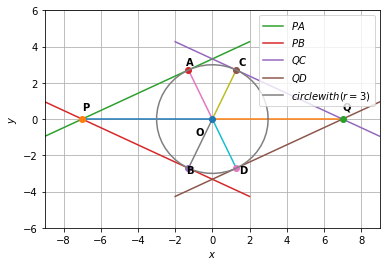
\includegraphics[width=\columnwidth]{FIGURE3.png}
    \caption{Tangent lines to circle of radius 3 units.}
    \label{fig:Tangent lines to circle of radius 3 units.}
\end{figure}
\end{enumerate}
\end{document}
